%TITULO------------------------------------------------------------------------

%==============================================================================
\chapter{Introdução}\label{introducao}
%==============================================================================

	%comentar sobre a conexão de conversores de tensão na rede e aplicações de filtragem
	%ativa. Depois, falar de geração distribuída e comentar problemas de harmônicas
	%de comutação

	A tensão fornecida pelo sistema elétrico de potência é idealmente senoidal e
	balanceada, com correntes de linha senoidais, amplitude e frequência fixas e
	fator de potência unitário. Durante a operação real do sistema, no entanto,
	é difícil manter as condições ideais. As divergências do padrão são classificadas
	como problemas de qualidade de energia e, por se tratarem de problemas, devem
	ser corrigidas.

	Problemas de qualidade de energia ocorrem com mais frequência e intensidade em
	ambientes industriais, devido ao tipo de carga instalada. Transformadores,
	fornos a arco, conversores tiristorizados e cargas semelhantes drenam correntes
	harmônicas e causam variações bruscas de energia reativa. É crescente a
	utilização de dispositivos eletrônicos de potência em equipamentos
	eletroeletrônicos, atualmente tão comuns em residências. Tais dispositivos possuem,
	em geral, um estágio de entrada sem correção do fator de potência, fazendo com que
	drenem correntes distorcidas da rede elétrica~\cite{ref:MANSOOR}. Estes fatores em
	conjunto agravam o problema de qualidade de energia, devido às suas consequências
	negativas, como	o aquecimento de condutores e transformadores devido à circulação
	de correntes reativas e o mau funcionamento de equipamentos sensíveis conectados
	ao sistema.	Tais consequências levaram à criação de normas internacionais que
	regulamentam limites para a distorção harmônica total, ou THD (do inglês \emph{
	Total Harmonic Distortion}). Como exemplos de normas pode-se citar a IEC 1000-3-2
	e a IEEE 519-1992.

	É possível mitigar estes problemas através da conexão de filtros de potência
	com a carga. Estes filtros podem ser ativos ou passivos, e a conexão pode ser
	em série, em paralelo, ou em série-paralelo. O filtro pode ser implementado
	com elementos passivos (resistores, indutores e capacitores) ou elementos
	ativos (chaves semicondutoras de potência), sendo os filtros ativos conhecidos
	como FAP's (Filtros Ativos de Potência). Embora filtros passivos sejam mais
	simples de projetar e mais baratos de construir do que filtros ativos, têm como
	desvantagem a possibilidade de oscilar com a impedância da linha e uma capacidade
	de compensação limitada, visto que para cada componente harmônica um reator
	deve ser projetado. Por isso, a partir da década de $70$, com o desenvolvimento
	da tecnologia de dispositivos semicondutores de potência, microprocessadores e
	processadores digitais de sinal, ou DSP's (do inglês \emph{Digital Signal
	Processor}) foi possível desenvolver algoritmos mais complexos de modulação,
	geração de referências e programas supervisórios, o que tornou a utilização de
	FAP's ainda mais popular~\cite{ref:SASAKI}.

	Além disso, diversos fatores têm levado à intensificação no uso de conversores
	eletrônicos	de potência nos últimos anos. As inúmeras aplicações que precisam de
	uma forma de conexão com a rede elétrica fazem uso de conversores de potência.
	Novas tecnologias, a crise energética e o aumento do efeito estufa são alguns dos
	motivos para o aumento desta demanda. Aplicações de geração distribuída, como
	células de energia,	painéis fotovoltaicos, turbinas eólicas e microturbinas são
	usadas não só para aumentar a energia disponível no sistema, mas também para
	melhorar sua confiabilidade, fornecendo energia aos consumidores mesmo durante
	uma falta na rede~\cite{ref:KARSHENAS}.	Na maioria destes geradores, a eletricidade
	está disponível em um estágio contínuo, ou é produzida em baixa frequência e,
	portanto, é convertida para um nível contínuo. Inversores de tensão são
	predominantemente utilizados para transferir energia de uma fonte contínua para
	a rede elétrica.

	Apesar de vastamente utilizados, os inversores de tensão demandam cuidado
	em sua utilização. Isso deve-se ao fato de o inversor de tensão trabalhar
	com uma frequência de comutação da ordem de $kHz$ para manter as perdas de
	comutação em níveis aceitáveis. Para manter as correntes harmônicas oriundas
	do inversor em níveis aceitáveis, de forma a respeitar os códigos de
	rede~\cite{ref:HOLMES}, existem diversas topologias de filtro que podem ser
	utilizadas~\cite{ref:RIBEIRO}. A mais comum é a aplicação de um filtro L como
	interface entre a rede e o inversor. Mais recentemente, filtros LCL começaram
	a ser utilizados para esta função~\cite{ref:LINDGREN}\cite{ref:TEODORESCU}
	\cite{ref:XU}, pois apresentam maior atenuação das frequências harmônicas sem
	aumentar significativamente o consumo de potência reativa na frequência
	fundamental da rede quando comparados a filtros L~\cite{ref:FUCHS}. Além disso,
	as dimensões do filtro LCL são significativamente menores que a de um filtro L,
	reduzindo o custo do filtro e as perdas de operação.

	A indutância da rede pode ser considerada como parte do filtro LCL. No entanto,
	a incerteza quanto ao seu valor real altera a frequência de ressonância do
	filtro e pode levar a instabilidade. Por este motivo, a incerteza quanto ao
	valor da indutância da rede precisa ser incluída no projeto do
	controlador~\cite{ref:LISERRE}. Outro ponto importante é que o controlador
	precisa rejeitar distorções de corrente de baixa ordem resultantes da
	distorção de tensão no ponto de conexão do conversor. Isto, aliado ao fato de
	que o controlador é implementado em um microcontrolador ou um DSP, torna o
	projeto bastante complexo.

	Por ser de terceira ordem, o filtro LCL apresenta um pico de amplitude em
	sua frequência de ressonância, o que faz com que a estabilidade geral do
	sistema seja reduzida dependendo principalmente de sua frequência de
	ressonância. Dessa forma, é necessário realizar o amortecimento deste pico
	de amplitude. É possível realizar este amortecimento de forma passiva
	através da inserção	de um resistor em série ou em paralelo com o capacitor
	do filtro~\cite{ref:AHMED}. Embora este amortecimento reduza consideravelmente
	o pico de amplitude na frequência de ressonância, ele aumenta o consumo de
	energia e degrada o desempenho do filtro nas altas frequências. Não é,
	portanto, uma solução aceitável para aplicações que necessitam do máximo de
	desempenho~\cite{ref:SHEN}. Outra forma de realizar este amortecimento é via
	amortecimento ativo. Isto é alcançado utilizando uma dentre várias estratégias
	de controle possíveis, tais como estruturas de controle específicas~\cite{ref:WU},
	estimação de impedância da rede~\cite{ref:BLAABJERG}, retroação de
	estados~\cite{ref:MASSING}, estratégias utilizando múltiplos laços de
	realimentação~\cite{ref:POH}, dentre outras~\cite{ref:WESSELS} \cite{ref:MORENO}
	\cite{ref:YANG}.

	Essas estratégias podem ser classificadas, de maneira geral, como analógicas
	e digitais. Os métodos de controle digital oferecem diversas vantagens sobre
	as técnicas analógicas, como reprogramabilidade, tolerância à variações
	nos componentes, suporte a multiplos modos de operação, melhor eficiência e,
	em geral, melhor desempenho. O controle analógico se limita a estruturas particulares,
	enquanto o controle digital depende apenas dos limites da taxa de amostragem,
	resolução e capacidade computacional~\cite{ref:KIMBALL}.

	Assim sendo, o enfoque recai sobre as técnicas de controle digital. Existem
	muitas técnicas diferentes para o controle de conversores. O controle
	proporcional-integral, comumente chamado de PI, utiliza compensadores de
	erro do tipo proporcional-integral para produzir os sinais de comando de
	cada fase. A parte integral do controlador minimiza o erro em baixas
	frequências, enquanto a parte proporcional e a posição do zero
	influenciam na ondulação do sinal. O desafio desta técnica é realizar o
	rastreamento das referências de corrente. Isto é resolvido, em geral,
	utilizando circuitos do tipo malha de captura de fase, ou PLL (do inglês
	\emph{Phase Locked Loop}) para gerar as referências de corrente. O controlador
	PI geralmente é implementado em eixos síncronos $dq$, de modo que as
	referências senoidais são transformadas em sinais constantes. Alternativamente,
	podem ser utilizados PI em eixos estacionários
	$\alpha \beta$~\cite{ref:KAZMIERKOWSKI}. Em ambos os casos, o objetivo é o
	rastreamento de referências senoidais e a rejeição de distúrbios de mesma
	natureza~\cite{ref:AREERAK}.

	Uma outra abordagem é o controle de corrente usando um controlador do tipo
	\emph{Dead-Beat}. Essa é a mais rápida estratégia de controle linear que pode
	ser adotada. Teoricamente, o laço de corrente replica exatamente a corrente
	de referência com dois ciclos de atraso. O controle é baseado no modelo interno
	da carga do conversor, usado para prever o comportamento dinâmico do sistema. O
	controlador, assim sendo, é inerentemente sensível a descasamento de parâmetros
	e de modelo~\cite{ref:MALESANI}.

	Existe ainda o controlador por Histerese. Devido à sua inerente não-linearidade,
	este controlador é capaz de proporcionar a mais rápida resposta dinâmica possível.
	Utilizando esta técnica, é possível atingir o máximo aproveitamento do conversor
	de potência~\cite{ref:YAO}. O limite para a regulação de corrente, na verdade,
	é dado pelo projeto do conversor. O controle de corrente por histerese é estável
	e robusto com relação à variações na carga ou qualquer outro tipo de distúrbios
	dinâmicos~\cite{ref:TENTI}.

	O controle de realimentação é a estratégia de controle mais simples que existe
	para compensar perturbações de um processo. Embora a grande maioria das estratégias
	de controle utilizadas na prática industrial seja controle de realimentação simples,
	essa estratégia apresenta uma desvantagem bastante significativa: é preciso que
	um distúrbio se propague pelo processo, fazendo a variável controlada desviar
	do ponto de operação, para que a realimentação adote uma ação corretiva~\cite{ref:SMITH}.

	Existem aplicações, no entanto, que demandam desempenho superior, devido à alguma
	necessidade específica, dinâmica lenta ou perturbações frequentes. Quando o distúrbio
	é associado à variável controlada ou quando o elemento de controle final apresenta
	comportamento não-linear, o Controle Multimalha melhora significativamente o
	desempenho em relação ao controle com realimentação simples~\cite{ref:KRISHNA}.

	Este tipo de controle pressupõe um conjunto de malhas em cascata, onde as mais
	externas geram as referências para as malhas mais internas. Dessa forma, variáveis
	intermediárias são usadas para reduzir o efeito de algumas dinâmicas no processo.
	Não é mais necessário esperar o distúrbio propagar-se pelo sistema e modificar a
	variável controlada. Uma vez que uma mudança seja detectada em uma variável
	intermediária, a ação corretiva começa imediatamente a ser aplicada na variável
	manipulada, reduzindo a magnitude do impacto do distúrbio e consequentemente
	melhorando o desempenho. O único requisito para que isto aconteça é que a malha
	interna seja mais rápida que a malha externa. Quanto mais rápida, melhor, pois
	a velocidade da malha interna implica na velocidade com que mudanças na variável
	intermediária serão detectadas, o que afeta diretamente a redução do impacto
	do distúrbio na variável controlada.

	As técnicas de controle clássicas pressupõe o uso de um modelo interno do sistema
	que deve ser precisamente conhecido. Nas duas últimas décadas, este requisito
	vem sendo relaxado, e o desafio é desenvolver estratégias de controle robustas
	à incerteza paramétrica~\cite{ref:GEROMEL}.

	%Considerando o contexto descrito acima, a proposta desse trabalho é apresentar
	%uma estratégia de controle de conversores conectados à rede elétrica através de
	%um filtro LCL. Esta estratégia apresenta ótimo desempenho através do uso de
	%Controle Multimalha, é capaz de rejeitar distúrbios e é robusta em relação à
	%incertezas paramétricas em termos da indutância da rede.

\section{Considerações sobre \emph{LCL}}

    A principal vantagem do filtro LCL sobre o filtro L é conseguir uma melhor
    atenuação das componentes harmônicas de corrente oriundas do processo de comutação do
    conversor utilizando componentes indutivos de menor volume. Isto é obtido pela
    inserção de um capacitor, resultando num filtro do tipo \emph{T}~\cite{ref:SHEN}.
    Para análise, considere a estrutura da Fig.~\ref{fig:LCL_topologia}. Os indutores
    $L_1$ e $L_2$ e o capacitor $C$ formam o filtro LCL, com suas resistências
    associadas $R_1$, $R_2$ e $R_d$ respectivamente. A indutância $L_g$ e sua
    resistência associada $R_g$ correspondem à indutância da rede, $V_i$
    é a tensão de saída do inversor e $V_g$ é a tensão da rede:

    \begin{figure}[htb]
        \centering{
            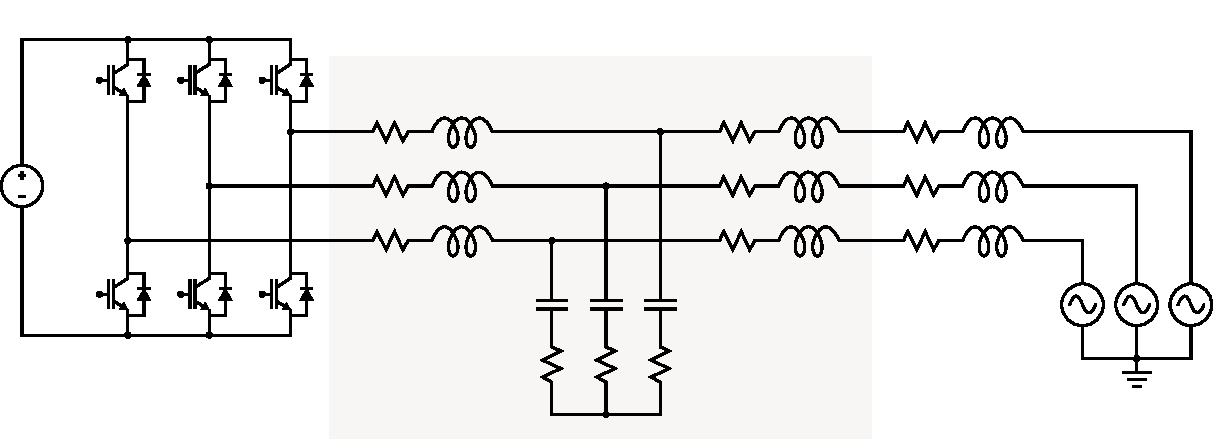
\includegraphics[width=0.9\textwidth]{img/topologia}}
        \renewcommand\figurename{Fig.}
        \caption{Topologia do filtro LCL.}
        \label{fig:LCL_topologia}
    \end{figure}

    Dessa forma, tem-se:

    \begin{equation*}
        Z_i = L_1s +R_1
    \end{equation*}

    \begin{equation*}
        Z_g = (L_2 + L_g)s + R_2 + R_g
    \end{equation*}

    \begin{equation*}
        Z_0 = \frac{1}{Cs} + R_d
    \end{equation*}

    Pode-se definir então, as seguintes funções de transferência:

    \begin{equation}
        G_{V_i-I_1}(s) = \frac{I_1(s)}{V_i(s)} = \frac{Z_g + Z_0}{Z_iZ_g + Z_iZ_0 + Z_gZ_0}
        \label{eq:G_v_i1}
    \end{equation}

    \begin{equation}
        G_{V_i-I_2}(s) = \frac{I_2(s)}{V_i(s)} = \frac{Z_0}{Z_iZ_g + Z_iZ_0 + Z_gZ_0}
        \label{eq:G_v_i2}
    \end{equation}

    \begin{equation}
        G_{I_1-I_2}(s) = \frac{I_2(s)}{I_1(s)} = \frac{Z_0}{Z_g + Z_0}
        \label{eq:G_i1_i2}
    \end{equation}

    Para efeito de comparação, pode-se reescrever a~(\ref{eq:G_v_i1})
    e~(\ref{eq:G_v_i2}) de forma a considerar apenas um indutor
    $L = L_1 + L_2 + L_g$. Negligenciando a resistência série do indutor,
    e considerando $\alpha = \frac{L_1}{L}$, têm-se:

    \begin{equation}
        G_{V_i-I_1}(s) = \frac{I_1(s)}{V_i(s)} = \frac{(1-\alpha)LCs^2+R_dCs+1}{\alpha(1-\alpha)L^2Cs^3+R_dLCs^2+Ls}
    \end{equation}

    \begin{equation}
        G_{V_i-I_2}(s) = \frac{I_2(s)}{V_i(s)} = \frac{R_dCs+1}{\alpha(1-\alpha)L^2Cs^3+R_dLCs^2+Ls}
        \label{eq:G_v_i2_2}
    \end{equation}

    \begin{figure}[htb]
        \centering{
            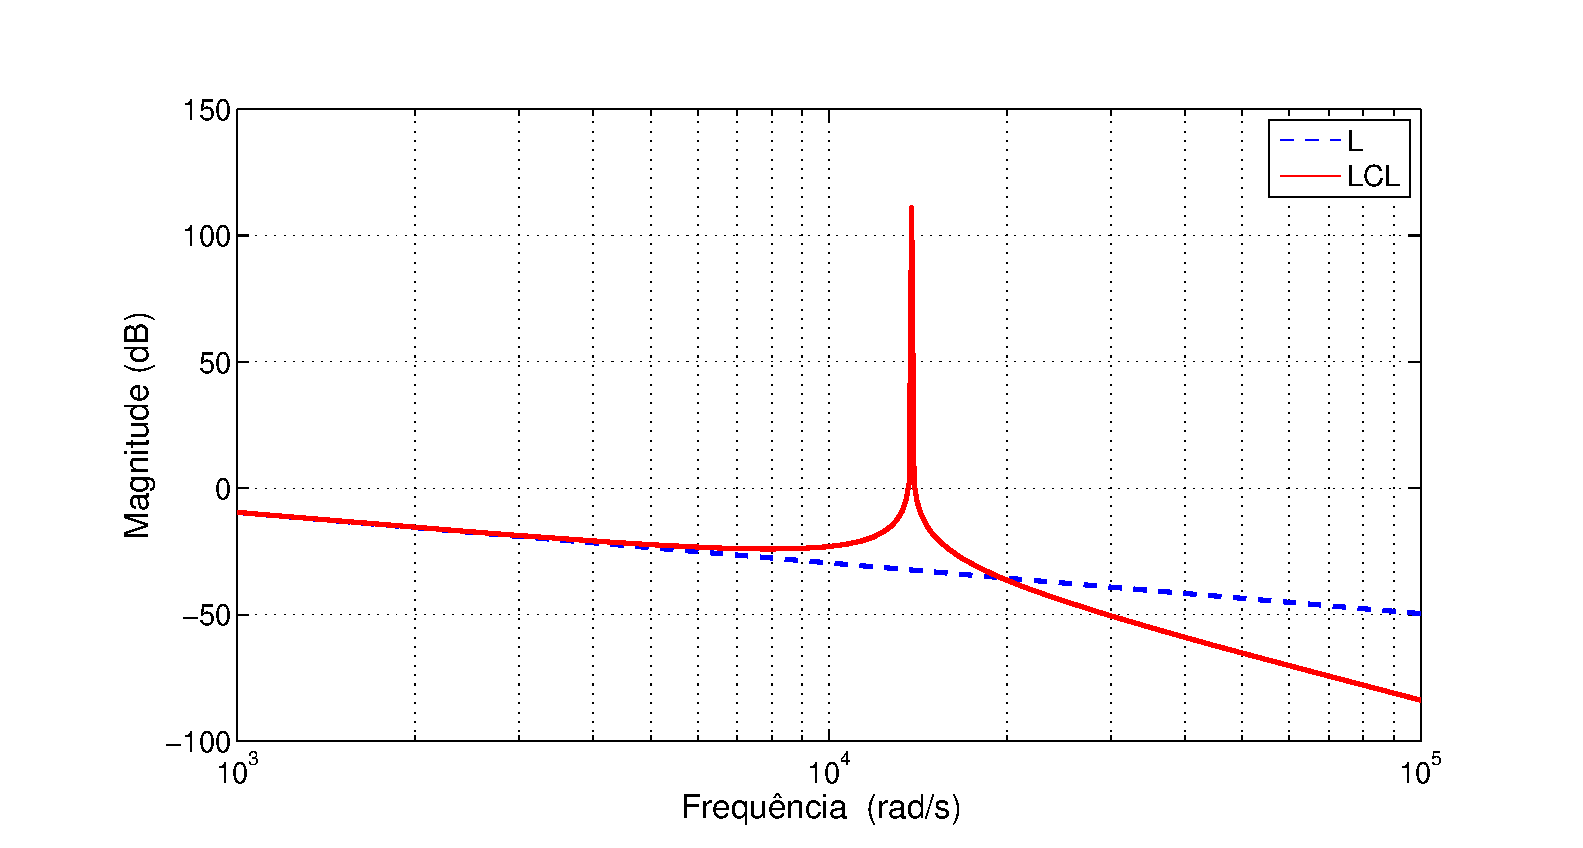
\includegraphics[width=0.9\textwidth]{img/L_vs_LCL}}
        \caption{Comparação entre filtro L e filtro LCL.}
        \label{fig:L_vs_LCL}
    \end{figure}

    A Fig.~\ref{fig:L_vs_LCL} mostra o diagrama de Bode de (\ref{eq:G_v_i2_2})
    com $R_d = 0$ para dois casos: com e sem capacitância $C$. No caso de $C = 0$,
    tem-se o filtro L. No caso de $C \neq 0$, tem-se o filtro LCL.

    Embora nos dois casos a indutância total tenha sido mantida a mesma, observa-se
    que o filtro LCL apresenta uma maior atenuação das harmônicas de comutação
    de alta frequência se comparado ao filtro L. Em contrapartida, o filtro LCL
    possui um pico de amplitude na frequência de ressonância. Por isso, é preciso
    mais cuidado no projeto para manter a estabilidade do sistema.

    O recurso mais comumente utilizado para tal é a adição de um resistor de
    amortecimento $R_d$. O amortecimento passivo, no entanto, prejudica a atenuação
    das harmônicas de alta frequência. A Fig.~\ref{fig:R_in_LCL} mostra o diagrama
    de Bode de (\ref{eq:G_i1_i2}) para $R_d = 0$, $R_d = 2\Omega$ e $R_d = 10\Omega$.

    \begin{figure}[htb]
        \centering{
            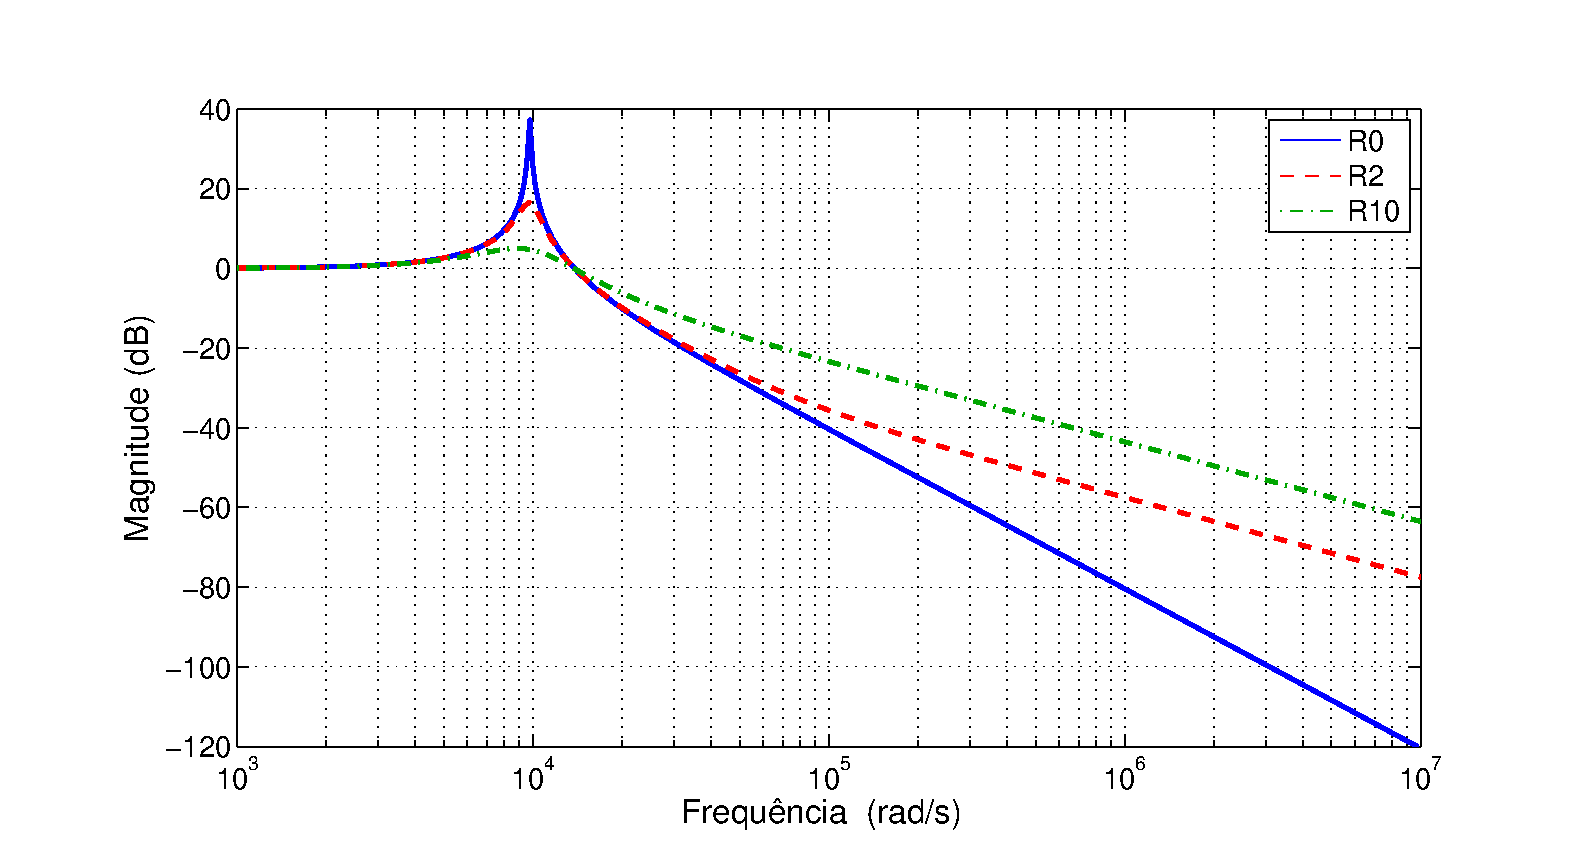
\includegraphics[width=0.9\textwidth]{img/R_in_LCL}}
        \caption{Diferença entre filtros L, LCL e LCL com amortecimento passivo.}
        \label{fig:R_in_LCL}
    \end{figure}

    A redução no amortecimento de harmônicas de alta frequência faz com que filtros
    LCL com amortecimento passivo sejam maiores que filtros LCL sem amortecimento
    passivo, para que atinjam o mesmo desempenho. Esse aumento de tamanho implica
    em aumento de custo e redução da banda passante do filtro. As considerações
    aqui feitas demonstram o porquê da escolha do filtro LCL sem
    amortecimento passivo. Embora seja mais trabalhoso e delicado projetá-lo,
    o desempenho é sensivelmente melhor.


\subsection{Corrente e Tensão do Capacitor}

    O sistema formado pelo conversor alimentado por tensão conectado à rede através
    de um filtro \emph{LCL} é um sistema composto por estados que podem ser
    utilizados em uma estrutura multimalha, onde a malha interna pode ser projetada
    para controlar a tensão ou a corrente do capacitor. Independentemente de qual
    variável é escolhida, o conhecimento da indutância $L_1$ e da capacitância $C$
    do filtro facilitam o projeto da malha interna. Deve haver, no entanto, capacidade
    de rejeição de distúrbios.

    %Comentar que independente de se controlar a tensão ou corrente do capacitor,
    %estas variáveis estão associadas a elementos conhecidos (L1 e C)

    O Controle Multimalha é adequado para melhorar o desempenho
    de sistemas de controle com apenas uma malha em que o distúrbio esteja
    relacionado com a variável manipulada ou quando o elemento de controle final
    exibe um comportamento não-linear~\cite{ref:LEE}.

    A Fig.~\ref{fig:multiloop} mostra a estrutura geral do Controle Multimalha, onde
    $r_1$ é a referência para a malha externa, $r_2$ é a referência para a malha
    interna, $G_p$ é a função de transferência do controlador primário,
    $G_s$ é a função de transferência do controlador secundário, $P_1$ e $P_2$
    são a planta, $d_1$ e $d_2$ são os distúrbios.

    %Uma forma
    %de fazer isto é controlar ou a corrente ou a tensão do capacitor. O controle
    %de cada parâmetro tem vantagens sobre o controle do outro, e é necessária
    %uma análise mais aprofundada para verificar qual a melhor opção.

    \begin{figure}[htb]
        \centering{
            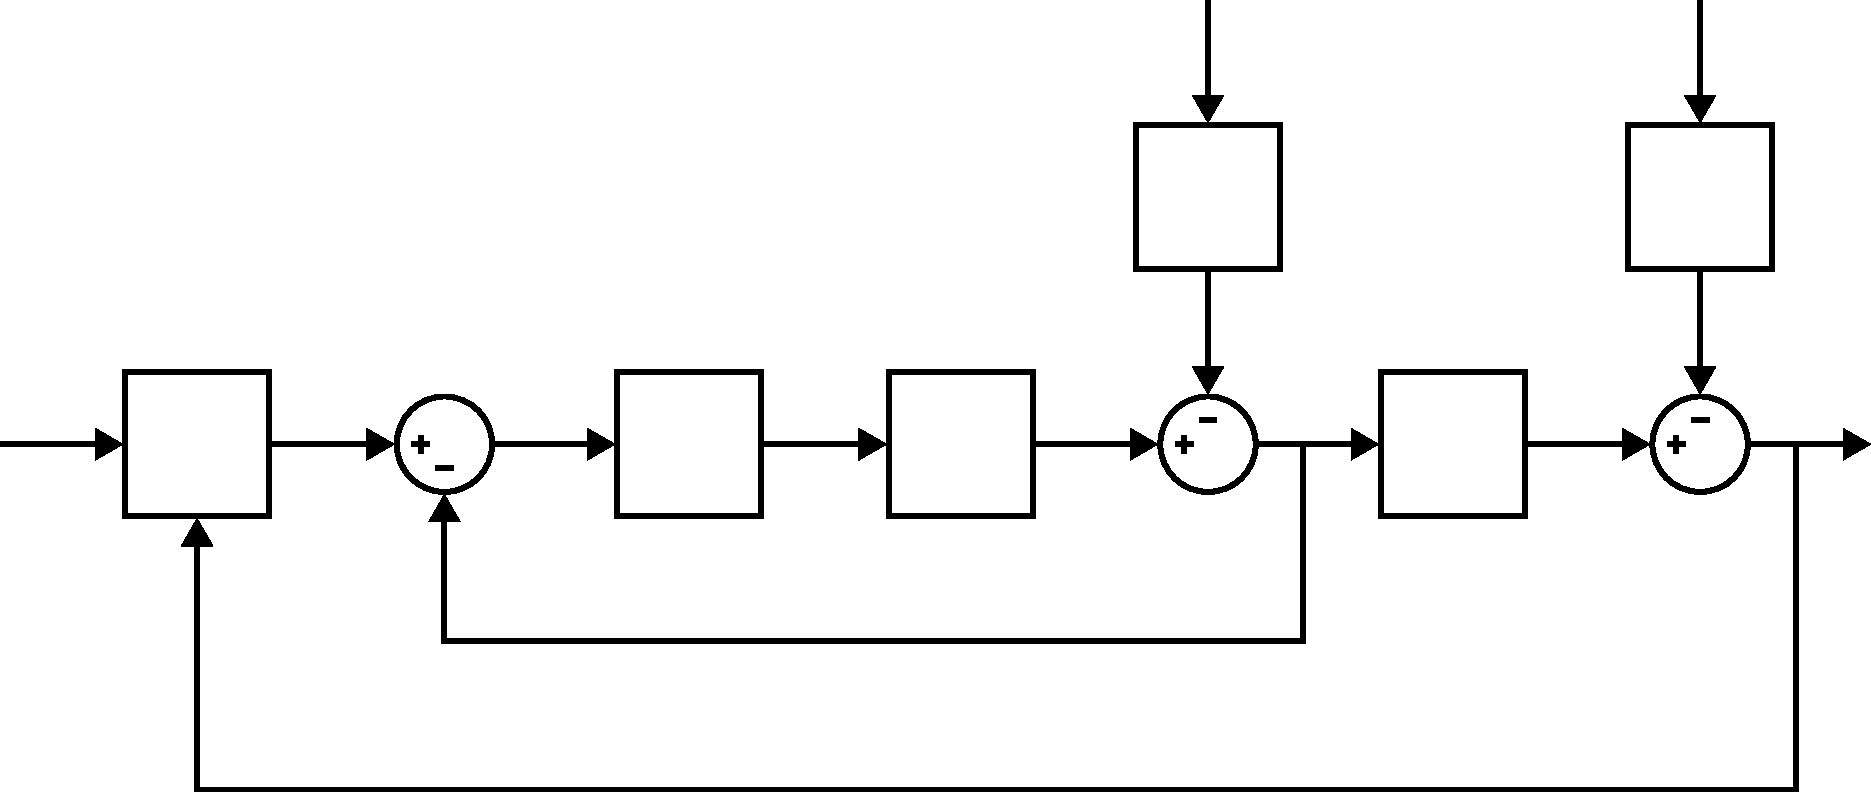
\includegraphics[width=0.9\textwidth]{img/multiloop_geral}}
        \renewcommand\figurename{Fig.}
        \caption{Estrutura geral de Controle Multimalha.}
        \label{fig:multiloop}
    \end{figure}

    A decisão sobre qual variável deve ser controlada em cada uma das malhas é complexa,
    e uma análise mais profunda deve ser feita para verificar qual a melhor
    opção para cada malha. Essa análise é feita em~\cite{ref:NASER}, utilizando o
    método do lugar das raízes e a técnica do espaço de estados médio. Esta é uma técnica
    essencial para a análise de circuitos chaveados, pois permite que as técnicas de
    análise de circuitos tradicionais sejam aplicadas à eles.

    O princípio de funcionamento é que a comutação ciclo à ciclo é ignorada em
    favor das características médias do circuito nas frequências abaixo da
    frequência de Nyquist. Perde-se então a capacidade de ver a forma de onda
    da comutação, mas pode-se determinar rapidamente uma série de fatores
    do circuito, como estabilidade, margem de ganho e de fase, o lugar das
    raízes e a resposta transiente média. Os passos para usar esta técnica são
    os seguintes:

    \begin{enumerate}
        \item Desenhar o circuito em cada estado;
        \item Escrever a equação de nó, malha ou elemento para cada estado;
        \item Determinar qual parcela do período o sistema permanece em cada estado;
        \item Multiplicar cada equação de estado por sua parcela de tempo e somá-las
            para obter uma média ponderada das equações de estado.
    \end{enumerate}

    As funções de transferência da tensão $v_c$ e da corrente $i_c$ do
    capacitor são dadas por:

    \begin{equation}
        v_c = \frac{\frac{2V_{DC}}{L_1} \frac{1}{C} \left( s + \frac{R_2}{L_2} \right)}{s^3 + a_2 s^2 + a_1 s + a_0}
        \label{eq:vc}
    \end{equation}

    \begin{equation}
        i_c = \frac{\frac{2V_{DC}}{L_1} s \left( s + \frac{R_2}{L_2} \right)}{s^3 + a_2 s^2 + a_1 s + a_0}
        \label{eq:ic}
    \end{equation}

    Com

    \begin{equation*}
        a_2 = \frac{R_1}{L_1} + \frac{R_2}{L_2}
    \end{equation*}

    \begin{equation*}
        a_1 = \frac{1}{L_1 L_2} \left( R_1 R_2 + \frac{L_1 + L_2}{C} \right)
    \end{equation*}

    \begin{equation*}
        a_0 = \frac{R_1 + R_2}{C L_1 L_2}
    \end{equation*}


    A Fig.~\ref{fig:rlocus_vc} mostra o lugar das raízes para a função de
    transferência (\ref{eq:vc}).

    \begin{figure}[htb]
        \centering{
            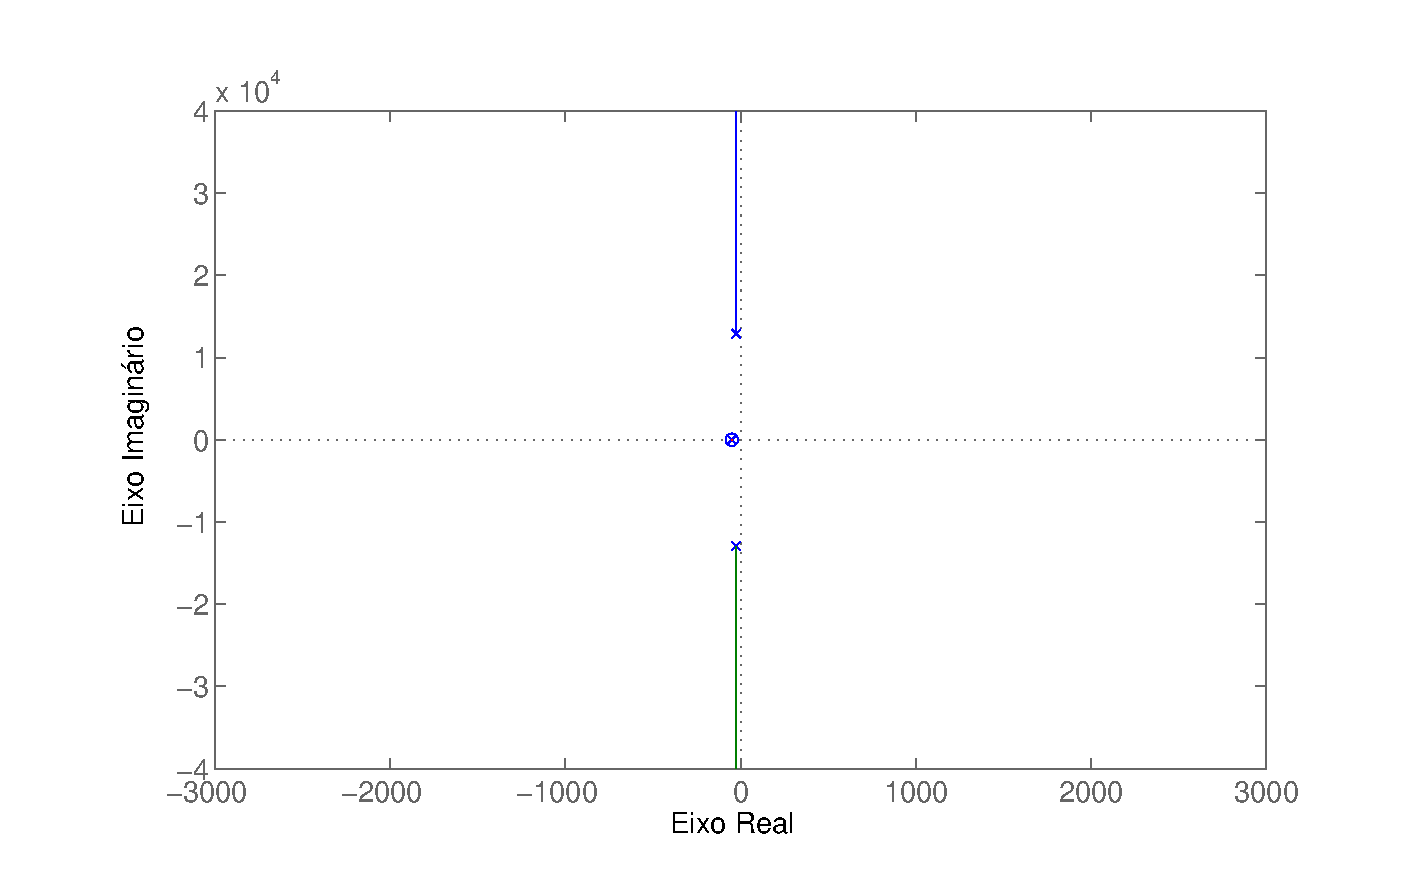
\includegraphics[width=0.9\textwidth]{img/rlocus_vc}}
        \renewcommand\figurename{Fig.}
        \caption{Lugar das raízes para a tensão do capacitor.}
        \label{fig:rlocus_vc}
    \end{figure}

    Percebe-se que os polos da função de transferência da tensão do capacitor
    apresentam um comportamento oscilatório ao longo do eixo imaginário. Devido
    ao projeto do filtro \emph{LCL}, a oscilação não ocorre em uma frequência
    muito alta, o que simplifica o controle desta variável. Além disso, na prática
    haverá sempre parte real nas resistências, o que fará com que os polos desloquem-se
    um pouco para o semiplano esquerdo, saindo do limiar de estabilidade.

    Supondo que o controlador da malha interna tenha um elevado desempenho
    no rastreamento de referências e na rejeição de distúrbios,
    o controle da tensão do capacitor é vantajoso. O capacitor
    pode ser visto como uma fonte de tensão, e toda a dinâmica
    do inversor e do indutor do lado do conversor podem ser ignorados,
    simplificando o controle da corrente da rede.

    A Fig.~\ref{fig:rlocus_ic} mostra o lugar das raízes para a função de
    transferência (\ref{eq:ic}).

    \begin{figure}[htb]
        \centering{
            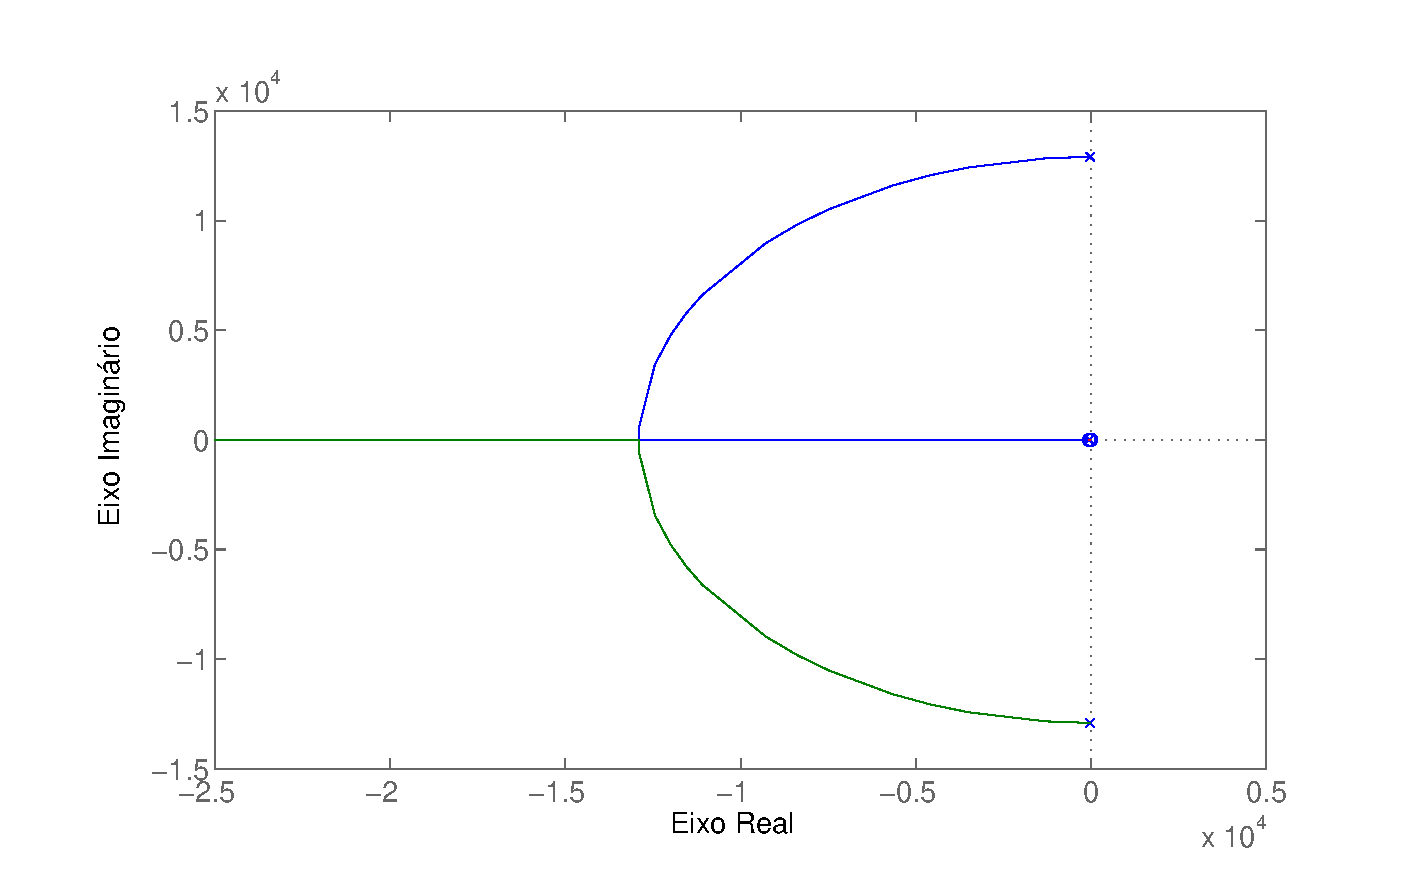
\includegraphics[width=0.9\textwidth]{img/rlocus_ic}}
        \renewcommand\figurename{Fig.}
        \caption{Lugar das raízes para a corrente do capacitor.}
        \label{fig:rlocus_ic}
    \end{figure}

    Percebe-se que os polos da função de transferência da corrente do capacitor
    deslocam-se para o semiplano esquerdo, indicando que o sistema tende à
    estabilidade. Essa é a grande vantagem de utilizar a corrente do capacitor
    como variável de controle da malha interna.

    A corrente do capacitor mostra-se como uma ótima escolha. No entanto, a tensão
    do capacitor pode ser selecionada como uma variável intermediária a ser controlada,
    sintetizando-se assim uma fonte de tensão controlada por tensão, no caso, o
    conversor. Deste modo, tem-se um circuito do tipo \emph{RL} que aproxima o
    comportamento no ponto de conexão.

    %Dessa forma, embora a corrente ofereça mais estabilidade, a tensão do capacitor
    %é escolhida como variável de controle da malha interna na presença de um controlador
    %adaptativo na malha externa, devido ao quanto essa escolha facilita a realização do
    %controle da dinâmica do filtro. Outras topologias para a malha externa serão
    %avaliadas, e então a corrente do capacitor será utilizada como variável de
    %controle para a malha interna.


\section{Objetivos e Contribuições da Dissertação}

	O objetivo desse trabalho é propor uma estratégia de controle para um conversor
	conectado à rede elétrica através de um filtro LCL. A estratégia proposta deve
	ser robusta com relação às incertezas e distúrbios da rede elétrica, e resultar
	numa dinâmica de malha fechada rápida o suficiente para permitir a rejeição de
	distúrbios e o rastreamento de possíveis referências complexas, incluindo harmônicas.

	Mais especificamente, esta Dissertação visa:

	\begin{itemize}
		\item Propor um controlador adaptativo para controlar a corrente de conversores
			conectados à rede elétrica com um filtro LCL que ajuste automaticamente os
			ganhos e que garanta estabilidade para uma ampla faixa de valores de
			impedância da rede;
		\item Propor um controlador que garanta desempenho e estabilidade frente a
			distúrbios de tensão e incerteza na impedância da rede elétrica;
		\item Realizar a prova de estabilidade do controlador proposto.
	\end{itemize}


\section{Organização do Documento}

	O Capítulo 1 apresenta a motivação para este trabalho. É apresentada uma breve
	revisão bibliográfica, de modo a situar o trabalho desenvolvido no contexto atual
	de utilização de conversores conectados à rede elétrica.

	O Capítulo 2 apresenta a modelagem matemática do sistema. O filtro LCL é modelado
	tanto em tempo contínuo quanto em tempo discreto, considerando como variável
	intermediária tanto a corrente como a tensão do capacitor.

	O Capítulo 3 apresenta a proposta de controlador adaptativo utilizando uma
	estrutura multimalha, novamente para ambos os casos de escolha de variável
	intermediária.

	O Capítulo 4 apresenta a prosposta de controlador adaptativo através de
	modelo interno.

	O Capítulo 5 apresenta os resultados obtidos com os controladores propostos,
	tanto em simulação quanto em experimentos de bancada.

	O Capítulo 6 traz as conclusões do trabalho e sugestões de trabalhos futuros.

%FIM---------------------------------------------------------------------------
